%%%----------------------------------------------------------
\chapter{2D Shape Signatures}
%%%----------------------------------------------------------

%TODO 05 implementation needed

The Contour Points Distribution Histogramm (CDPR) method uses  a shape's contour points as its description. The shape is separated into a circular reference grid consisting of $n_R$ radial and and $n_A$ axial subdivisions. The center of the grid is aligned to the shape's centroid which makes the descriptor translation-invariant. The radius of the out circle is defined by the most distant contour point. Then each subdivision of this reference grid gets mapped to a distribution histogram field. The histogram is calculated by assigning each contour point to the respective segment. By normalizing the histogram the descriptor gets scale-invariant. To make the descriptor also rotation-invariant use the major axis of the shape.

This assignment consist of two parts. In the first part CPDH algorithm needs to be implemented. In the second part this implementation is used to match shapes comparing their histograms.

\section{Construction of the original CPDH "shape signature"}
To create CPDH signature the following steps were executed:
\begin{enumerate}
	\item Calculate the centroid of the shape $x_c$. This will be used as center of the reference grid.
	\item Find the contour point which is the furthest away from the centroid and use the distance to define the radius of the reference grid.
	\item Setup the rest of the reference grid by dividing it in $n_A$ axial and $n_R$ radial subdivisions.
	\item Create the associated histogram with a dimension of $n_A \cdot n_R$.
	\item Find the respective histogram bin for each contour point and increase the bin count.
	\item Normalize the histogram values ($\sum B_{i,j} = 1$).
\end{enumerate}

\subsection{Creating the reference grid}
As already mentioned the centroid of the shape was used as center of the reference grid and the distance to point the furthest away from the center as radius for to outer circle. To draw the lines for axial separation fo the circle a vector from the center to the top point of the outer circle is created then it is rotated $n_A -1$ times for $360/n_A$ degrees and drawn.

The radius for additional circles for the reference grid is calculated by dividing the radius of the outer circle by $n_R$.

\subsection{Calculate histogram values}
To be able to map contour points from the reference grid to the the radial $i_R$ and angular $i_A$ index had to be calculated:
\begin{itemize}
	\item For calculating $i_A$ two vectors were created. The vector between the center and the current contour point $P$ as well as the vector between the center and the top point of the outer circle. Then the angle these vectors is calculated and divided by $360/n_A$ after that $2\cdot \pi$ has to be added to avoid negative values.
	\item To calculate $i_R$ the distance between the center and the contour point is calculated and then divided by the circle radius step size ($r_c/n_R$) and the outcome limited to $n_R -1$ to avoid $i_R = n_R$.
\end{itemize} 

\begin{figure}
	\centering
	\frame{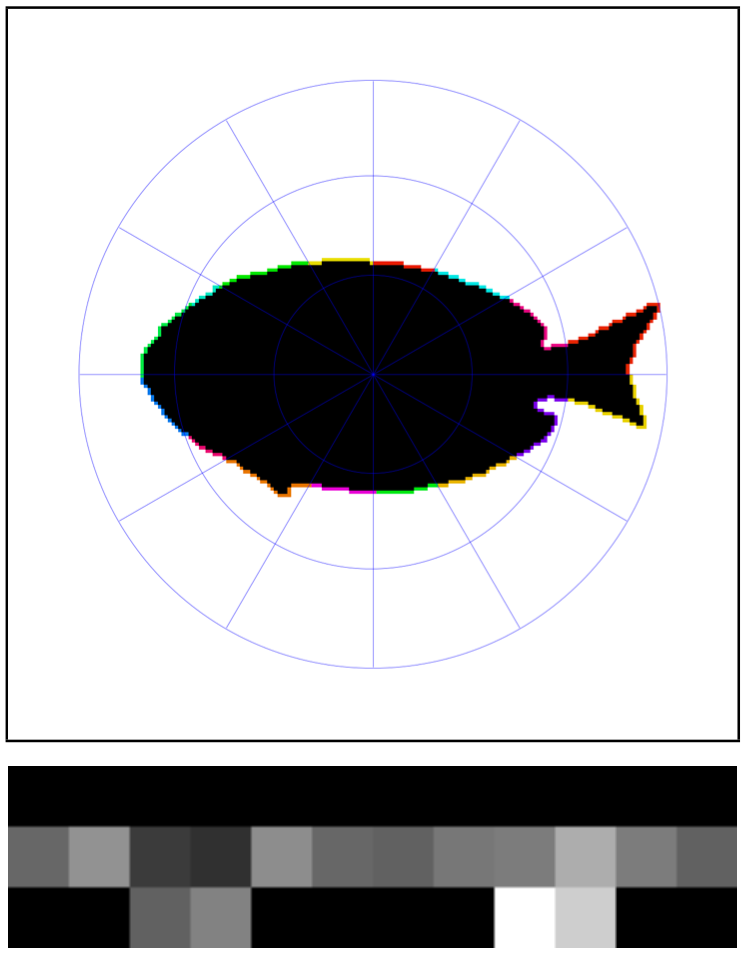
\includegraphics[width=0.4\linewidth]{images/ass05_grid}}
	\caption{Shape with reference grid and calculated histogram.}
	\label{fig:Result5_1}
\end{figure}

\subsection{Adding rotation invariance}
At the moment rotating the shape would lead to a shift of the histogram. To make the histogram rotation-invariant the rotation of the shape needs to be calculated and the reference grid aligned accordingly. For the calculation of the orientation $\theta$, central moments $\mu_{pq}$ are used.

\begin{equation}
	\theta = \frac{1}{2} \cdot \tan^{-1}\left(\frac{2 \cdot \mu_{11}}{\mu_{20} - \mu{02}}\right)
\end{equation}

\begin{equation}
	\mu_{pq} = \sum_{(u,v) \in \R} (u-\overline{x})^p \cdot (v - \overline{y})^q
\end{equation}

Now when drawing the reference grid the orientation is added to the angle and we also need to keep it in mind when calculating the angular index $a_R$.

\begin{figure}
	\centering
	\frame{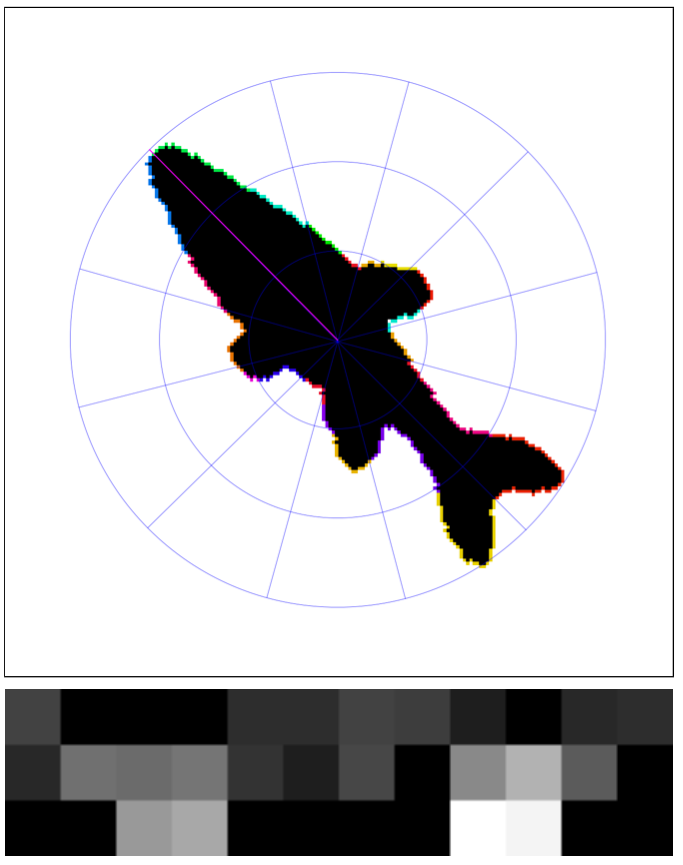
\includegraphics[width=0.4\linewidth]{images/ass05_major}}
	\caption{Added rotation invariance.}
	\label{fig:Result5_6}
\end{figure}

\section{Shape signature matching}
For matching a number of shapes to a set of reference images the following steps have been executed:
\begin{enumerate}
	\item Create CPDH for all reference shapes.
	\item Calculate CDPH for all detected shapes.
	\item Use the L2 distance to calculate the closest reference image for each detected shape.
	\item Mark similar shapes with the same rectangle color.
\end{enumerate}

As we can see in figure \ref{fig:Result5_3} the shape matching worked pretty well all reference shapes (figure \ref{fig:Result5_2}) were detected. All shapes which were only transformed or rotated were detected while if they were mirrored they waere not. 

\begin{figure}
	\centering
	\frame{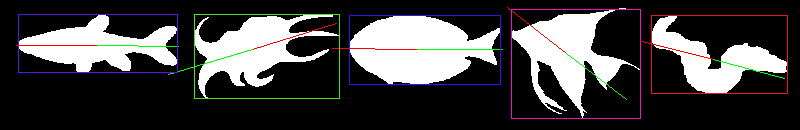
\includegraphics[width=0.8\linewidth]{images/ass05_ref}}
	\caption{Reference shapes}
	\label{fig:Result5_2}
\end{figure}

\begin{figure}
	\centering
	\frame{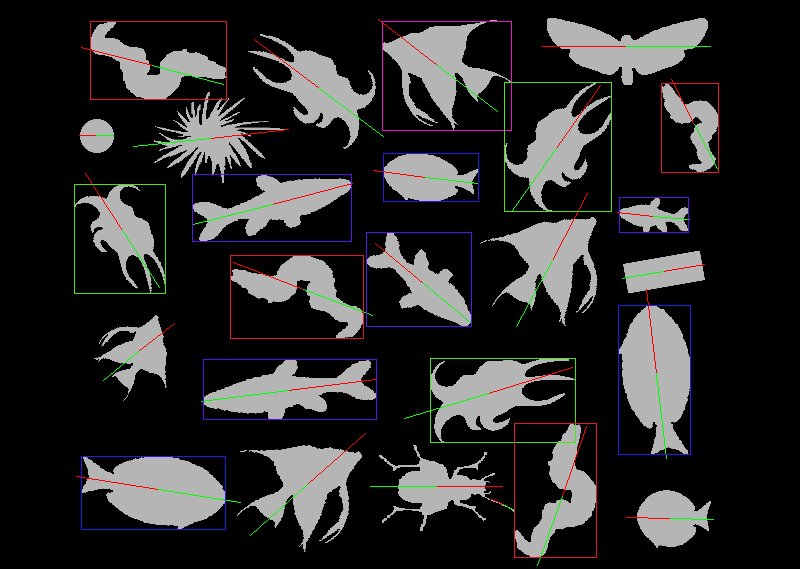
\includegraphics[width=0.8\linewidth]{images/ass05_matching}}
	\caption{Result of shape matching with their reference shapes from \ref{fig:Result5_2}.}
	\label{fig:Result5_3}
\end{figure}